%!TEX root = thesis.tex
\hypertarget{functions---constant-generators}{%
\section{Functions - constant
generators}\label{functions---constant-generators}}

The following functions are from `AES\_encrypt\_generator.py' No
function in the following chapter does error checking, since they are
only intended for use inside a static, unchanging setting.

\hypertarget{galois-field-multiplication-lookup-table-generator}{%
\subsection{Galois field multiplication lookup table
generator}\label{galois-field-multiplication-lookup-table-generator}}

\hypertarget{description}{%
\subsubsection{Description}\label{description}}

As \cite{rijndael} recommends in chapter 4.1.1 Galois field multiplications
used in MixColumns were implemented as lookup tables in the Galois field multiplication lookup table (GFMLT). Since the
number of possible multiplication results is highly restricted in $GF(2^{8})$
the table storing all results uses negligible memory. This avoids computing
the multiplications over and over. Furthermore in chapter 10.8.1 the
authors suggest, that implementing the multiplications as table lookups
makes the algorithm more resistant to timing attacks, since the finite
field multiplication performed in MixColumns is the only operation in
Rijndael that is not computed in constant time. In their 8-bit
implementation in chapter 4.1.1 they suggest only generating a table t
where table t[a] = 02 * a, since multiplication with one is the factor
itself and multiplication with three can be efficiently archived by
XORing the result of the multiplication with two with the original
number: 03 * a = (02 * a) xor a

To avoid leaking more timing data than
absolutely necessary the present implementation uses a lookup table for
all values, since this ensures that for each multiplication the CPU
(theoretically) does always the exact same amount of work, thus ensuring
it always takes the exact same amount of time. This size increase by 2 *
256b = 512 bytes (compared to the suggested implementation with only one
row) is negligible for our target of x86-CPU-systems, which today
typically feature memory sizes in the gigabyte range.

\cite{rijndael} did not
make a mistake in their implementation suggestion though, since the
small lookup table variant was only suggested for memory constrained
8-bit environments. For 32-bit-architectures or wider they make even more
extensive use of lookup tables than the present implementation does
(compare ch. 4.2). This variant has not been used, since it reduces the
steps of the algorithm for each column in each round into four table
lookups accessing large tables crafted for this purpose, and four XOR
operations concatenating the lookup-results. This obscures the original
layout of the algorithm heavily and it was decided, that it should it to be recognizable
in the present implementation.

In the end the suggestions \cite{rijndael} makes regarding this topic have to
be taken with a grain of salt, since the extensive use of lookup tables
seems to enable new side channel attack vectors as previously discussed in the thesis.

The lookup table used by the present implementation extends over two
dimensions: three rows for the multiplicands one, two and three and 256
columns to store the results of the multiplications with the numbers
denoting the column indices. Since the first dimension denotes the
multiplicator m, m - 1 accesses the right array for multiplication with
m, while the second dimension accesses the result for the value wanted.

\begin{quote}
The program needs to compute the multiplication of two times 114. This
means it has to access gal\_mult\_lookup[2-1]. For the result it
simply needs to use the second factor as the array index for the second
dimension. Thus the final array access to calculate 2 * 114 in $GF(2^{8})$ is
gal\_mult\_lookup[1][114]. For 3 * 86 it would be
gal\_mult\_lookup[2][86] etc.
\end{quote}

\hypertarget{implementation}{%
\subsubsection{Implementation}\label{implementation}}

\begin{lstlisting}
def mult_gal(a, b):
    """
    Multiplicates two numbers in the Galois Field specified by the AES-Standard.

    Algorithm specified under
    https://en.wikipedia.org/wiki/Finite_field_arithmetic#multiplication
    as a modiefied version of the "peasant's algorithm"
    Tested with https://www.ece.unb.ca/cgi-bin/tervo/calc2.pl
    """

    p = 0
    for i in range(8):
        if (a == 0) or (b == 0):
            break
        if b & 1:
            p ^= a
        b >>= 1
        a = ((a << 1)%256) ^ (-(a >> 7) & 0x1b)
    return p
\end{lstlisting}

This implementation of multiplication in $GF(2^{8})$ modulo $m(x) = x^8 + x^4 +
x^3 + x + 1$ is an adapted version from the `peasant's algorithm' as
described in
\cite{peasants}.
It takes two integers with values in range of 0-255 `a' and `b'. First
the variable `p' gets initialized with 0. The following loop gets
repeated at most eight times: If one of the two factors is 0 the
algorithm terminates. After that, `mult\_gal' evaluates, whether `b' is
odd by performing a bitwise AND-operation with `b' and 1. If the least
significant bit of `b' was toggled `p' gets XORed with `a' and the
result is stored in p. After that `b' gets bitshifted one to the right,
which equals division by two while ignoring the remainder. The last step
has two components.
The first component shifts 'a' to the right by one and cuts off any byte overflow
by using the modulo function. If such overflow occured, the modulo operation has to be
applied to the shifted 'a' in order to keep in in $GF(2^{8})$. This is done by XORing it
with m(x) which is 100011011 in binary and 1b in hexadecimal, when fit into a byte (because
this removes the most significant digit of m(x)). To detect overflow 'a' is shifted to the right by 7
and then negated. If the most significant bit of 'a' was set (which means overflow), 1b gets ANDed
with -1 or 11111111 in binary (due to the two's complement), thus resulting in the modulo being applied to the doubled 'a'. In the other case 1b gets ANDed with 0, which results in the second term getting cancelled out, resulting in a simple doubling of 'a'.

'gen\_mult\_lookup()' then uses the function to generate the values for
multiplication of all numbers in $GF(2^{8})$ with two and three.

The results (\ref{t:GFMLT}) were spot-checked against
\cite{galcalc} with P(x) = 100011011.

\hypertarget{s-box-generator}{%
\subsection{S-box generator}\label{s-box-generator}}

\hypertarget{description-1}{%
\subsubsection{Description}\label{description-1}}

The S-box generator is used to generate the S-box needed in the
SubBytes-function.
The values of the AES S-box are computed by taking the value of the byte
that needs to be substituted, finding its inverse in $GF(2^{8})$ with the
irreducible polynomial $m(x) = x^8 + x^4 + x^3 + x + 1$ and applying an
affine transformation to that inverse. (\cite[ch 3.4.1]{rijndael})

\begin{figure}
\centering
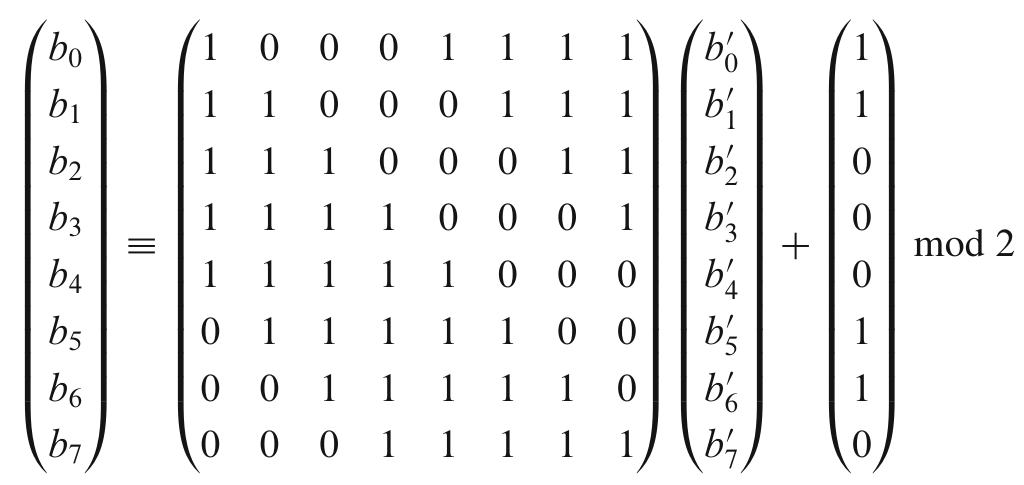
\includegraphics[scale = 0.3]{data/figures/affinetrans.png}
\caption{The affine transformation used in the AES S-box depicted as a matrix multiplication.}
\end{figure}

The S-box contains a substitution for every value an unsigned byte is
able to contain. \ref{t:sbox} shows the S-box filled with values (in
hexadecimal) the present implementation generates. To use it in this
table format one has to split the byte to substitute into its digits.
The most significant digit is used to look up the row, the least
significant shows the column in that row. The intersection shows the
substitution value.

\begin{quote}
The byte to substitute contains the hexadecimal value of b8. The most
significant digit is b, meaning the substitution value is located in the
b-row. The least significant digit is 8, meaning the substitution value
is located in the 8-column of the table. Therefore the substitution
value is 6c, because it is located, where the b-row and the 8-column
intersect each other.
\end{quote}

\hypertarget{implementation-1}{%
\subsubsection{Implementation}\label{implementation-1}}

\begin{lstlisting}
def mult_inv_gal():
    """
    Generates a table of the multiplicative inverse of the Elements
    contained within the AES-Galois-Field.

    It uses an unelegant brute-force-method.
    """
    list_start = [*range(1, 256)]
    list_res = [0]
    for i in range(256):
        for j in list_start:
            if mult_gal(i, j) == 1:
                list_res.append(j)
                list_start.remove(j)
    return bytearray(list_res)
\end{lstlisting}

This function generates the inverses for all values in $GF(2^{8})$. First it
generates a list with the values from 1 to 255. After that it creates
another list containing the element 0 (since 0 has no inverse). Now it
iterates through all 256 possible values p. For each p it goes through
`list\_start' and multiplies them in $GF(2^{8})$ modulo m(x) using the
previously mentioned `mult\_gal' function. Since multiplying a number x
with its inverse always results in the multiplicative identity 1, the
present implementation simply tries to multiply all elements in $GF(2^{8})$
with each other (basically a brute-force approach) to see if the product
equals 1. In that case the value r from `list\_start' is appended to
`list\_res' at the index of the current value of p. After that r is
removed from list\_start, since every p has only one inverse in $GF(2^{8})$
modulo m(x). In the
end the function returns `list\_res' converted to a byte array,
containing numbers that are the inverses of the values of their indices
(eg. element at list index 37 is the inverse to the number 37).
The result of the function was compared against \cite[Table A.5.]{rijndael} to verify
correctness.

\begin{lstlisting}
def shift_left(byte, rot):
    """Implements a left bitwise circular shift for bytes."""
    temp = (byte << rot)%256
    byte = temp | ((byte >> (8-rot)))
    return byte
\end{lstlisting}

This function implements a left bitwise circular shift of a byte. It
takes two arguments, `byte' and `rot'. `byte' is an integer in the range
of 0-255 and rot is an integer, denoting the number of places `byte'
should be shifted by. It starts by applying a bitwise left shift to
`byte', shifting it `rot' times. The result is reduced by modulo 256,
since the result cannot leave the range denoted by an unsigned byte,
e.g. 0-255. The reduced result is placed into the variable `temp'. Now
the bits of `byte' that got shifted to the left and `cut off' by the
modulo operation have to be brought back to the right. For that we shift
`byte' 8 - `rot' bits to the right. Now the two `halves' get combined by
applying a bitwise OR to `temp' and the result of the right shift. This
result is saved in `byte'. Finally the function returns `byte'.

\begin{lstlisting}
def gen_sbox():
    """Genereates the AES S-box"""
    mult_inv_table = mult_inv_gal()
    sbox = bytearray(256)
    j = 0
    for i in mult_inv_table:
        #affine transformation
        sbox[j] = i ^ shift_left(i, 1) ^ shift_left(i, 2) ^ shift_left(i, 3) ^ shift_left(i, 4) ^ 0x63
        j += 1
    return sbox
\end{lstlisting}

This function generates the S-box array. First it uses the
`mult\_inv\_gal' function to generate a list containing all
multiplicative inverse of the elements in $GF(2^{8})$. After that it
allocates a byte array with length 256 called `sbox' and initializes the
variable `j' with zero. Then it iterates through the array of inverses,
applying the affine transformation and storing the result in sbox. The
affine transformation is computed by XORing the list element with
versions of itself that have been shifted left via circular byteshift
one, two, three and four times. Finally the result gets XORed with 99 to
obtain the result of the transformation.
(https://en.wikipedia.org/wiki/Rijndael\_S-box\#forward\_s-box) The
function finishes by returning the S-box-byte-array.

Since this is a static function generating always the same array, the
resulting array was compared once with the table in \cite[Fig. 7]{fips197}
